%!TEX program = xelatex
\documentclass[dvipsnames, svgnames,a4paper,11pt]{article}
% ----------------------------------------------------
%   吉林大学通信工程学院信号与系统实验报告
%   原作者:Huanyu Shi,2019级
%     知乎:https://www.zhihu.com/people/za-ran-zhu-fu-liu-xing
%     Github:https://github.com/huanyushi/SYSU-SPA-Labreport-Template
%   在原基础上魔改了一些,更加贴近吉林大学实验格式。
% ----------------------------------------------------

% ----------------------------------------------------- 
%	加边框的命令
%	参考:https://tex.stackexchange.com/questions/531559/how-to-add-the-page-border-for-first-two-pages-in-latex
\usepackage{tikz}
\usetikzlibrary{calc}
\usepackage{eso-pic}
\AddToShipoutPictureBG{%
\begin{tikzpicture}[overlay,remember picture]
\draw[line width=0.6pt] % 边框粗细
    ($ (current page.north west) + (0.6cm,-0.6cm) $)
    rectangle
    ($ (current page.south east) + (-0.6cm,0.6cm) $); % 边框位置
\end{tikzpicture}}


\usepackage{xcolor}
\definecolor{c1}{HTML}{2752C9} % 目录颜色
\definecolor{c2}{RGB}{190,20,83} % 引用颜色

\usepackage{ctex}
\usepackage[top=28mm,bottom=28mm,left=15mm,right=15mm]{geometry}
\usepackage{hyperref} 
\hypersetup{
	colorlinks,
	linktoc = section, % 超链接位置,选项有section, page, all
	linkcolor = c1, % linkcolor 目录颜色
	citecolor = c1  % citecolor 引用颜色
}
\usepackage{amsmath,enumerate,multirow,float}
\usepackage{tabularx}
\usepackage{tabu}
\usepackage{subfig}
\usepackage{fancyhdr}
\usepackage{graphicx}
\usepackage{wrapfig}  
\usepackage{physics}
\usepackage{appendix}
\usepackage{amsfonts}

%
\usepackage{tcolorbox}
\tcbuselibrary{skins,breakable}
\newtcolorbox{tbox}[2][]{
    colframe=black!70!,
    breakable,
    enhanced,
	boxrule =0.5pt,
    title = {#2},
    fonttitle = \large\kaishu\bfseries,
	drop fuzzy shadow,
    #1
}
\newtcolorbox[auto counter,number within=section]{question}[1][]{
  top=2pt,bottom=2pt,arc=1mm,
  boxrule=0.5pt,
%   frame hidden,
  breakable,
  enhanced, %跨页后不会显示下边框
  coltitle=c1!80!gray,
  colframe=c1,
  colback=c1!3!white,
  drop fuzzy shadow,
  title={思考题~\thetcbcounter:\quad},
  fonttitle=\bfseries,
  attach title to upper,
  #1
}

% ---------------------------------------------------------------------
%	利用cleveref改变引用格式,\cref是引用命令
\usepackage{cleveref}
\crefformat{figure}{#2{\textcolor{c2}{图 #1}}#3} % 图片的引用格式
\crefformat{equation}{#2{(\textcolor{c2}{#1})}#3} % 公式的引用格式
\crefformat{table}{#2{\textcolor{c2}{表 #1}}#3} % 表格的引用格式


% ---------------------------------------------------------------------
%	页眉页脚设置
\fancypagestyle{plain}{\pagestyle{fancy}}
\pagestyle{fancy}
\lhead{\kaishu 吉林大学通信工程学院} % 左边页眉,学院 + 课程
\rhead{\kaishu 信号与系统实验报告} % 右边页眉,实验报告标题
\cfoot{\thepage} % 页脚,中间添加页码


% ---------------------------------------------------------------------
%	对目录、章节标题的设置
\renewcommand{\contentsname}{\centerline{\huge 目录}}
\usepackage{titlesec}
\usepackage{titletoc}
% \titleformat{章节}[形状]{格式}{标题序号}{序号与标题间距}{标题前命令}[标题后命令]
\titleformat{\section}{\centering\LARGE\songti}{}{1em}{}

% ---------------------------------------------------------------------
%   listing代码环境设置
\usepackage{listings}
\lstloadlanguages{python}
\lstdefinestyle{pythonstyle}{
backgroundcolor=\color{gray!5},
language=python,
frameround=tftt,
frame=shadowbox, 
keepspaces=true,
breaklines,
columns=spaceflexible,                   
basicstyle=\ttfamily\small, % 基本文本设置,字体为teletype,大小为scriptsize
keywordstyle=[1]\color{c1}\bfseries, 
keywordstyle=[2]\color{Red!70!black},   
stringstyle=\color{Purple},       
showstringspaces=false,
commentstyle=\ttfamily\scriptsize\color{green!40!black},%注释文本设置,字体为sf,大小为smaller
tabsize=2,
morekeywords={as},
morekeywords=[2]{np, plt, sp},
numbers=left, % 代码行数
numberstyle=\it\tiny\color{gray}, % 代码行数的数字字体设置
stepnumber=1,
rulesepcolor=\color{gray!30!white}
}




% ---------------------------------------------------------------------
%	其他设置
\def\degree{${}^{\circ}$} % 角度
\graphicspath{{./images/}} % 插入图片的相对路径
\allowdisplaybreaks[4]  %允许公式跨页


%---------------------------------------------------------------------------%
%->> User defined commands
%---------------------------------------------------------------------------%
\RequirePackage{mathrsfs}% script style math symbols % 导入模板的相关设置
\usepackage{lipsum}


%---------------------------------------------------------------------
%	正文
%---------------------------------------------------------------------

\begin{document}

\begin{table}
  \raggedleft
	\renewcommand\arraystretch{1.7}
	\begin{tabular}{|c|p{4em}|}
	  \hline
	  成绩 &  \\
	  \hline
	  教师签字 &   \\
	  \hline
	\end{tabular}
\end{table}

\begin{center}
	{\kaishu \LARGE   \quad  \quad 通  \quad 信  \quad 工  \quad 程  \quad 学  \quad 院 }
  \newline
  \newline
  \newline
  \newline
  \newline
  {\kaishu \Huge 实 \quad  \quad  \quad 验  \quad  \quad  \quad 报 \quad  \quad  \quad 告}
  \newline
  \newline
  \newline
  \newline
  \newline
  {\songti \Huge  ( \quad  信  \quad 号  \quad 与  \quad 系  \quad 统 \quad)}
  \newline
  \newline
  \newline
  \newline
  \newline
  {\songti  \LARGE 实验题目:线性系统的频率特性  \quad  \quad \quad}
\end{center}



\begin{table}[b]
	\renewcommand\arraystretch{1.7}
	\begin{tabularx}{\textwidth}{|X|X|X|X|}
	  \hline
	  专业:& 通信工程 &年级:& 2022级\\
	  \hline
	  姓名:& 苏睿杰  & 学号:& 20220826\\
	  \hline
	  实验时间:& 2023年10月27日 & 班级:& 42 \\
	  \hline
	\end{tabularx}
\end{table}


%\clearpage
%\tableofcontents

\clearpage
\setcounter{section}{0}
\section{实验十九 \quad 线性系统的频率特性}
	
\subsection*{一、实验目的}
\begin{enumerate}
	\item 熟练掌握测频谱的方法。
	\item 加深对矩形脉冲频谱特点的掌握。
\end{enumerate}

\begin{figure}[htbp]
	\centering
	\subfloat[]{
		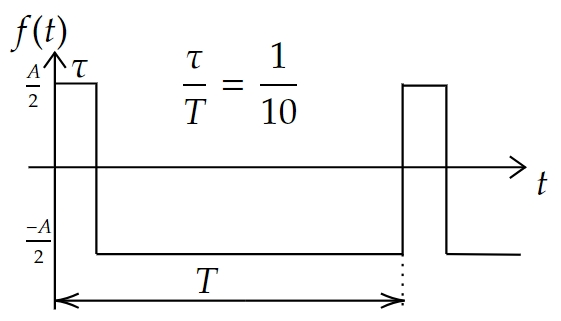
\includegraphics[width=0.4\textwidth]{3.18.1(a).png}
	}
	\subfloat[]{
		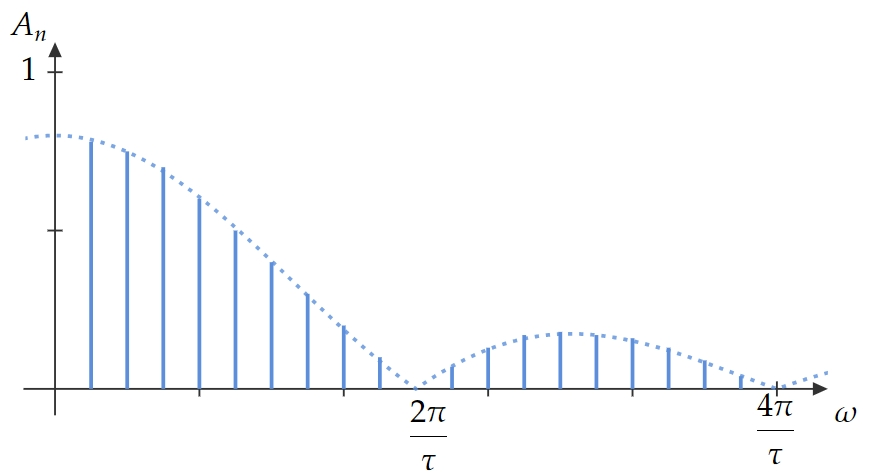
\includegraphics[width=0.45\textwidth]{3.18.1(c).png}
	}

	\subfloat[]{
		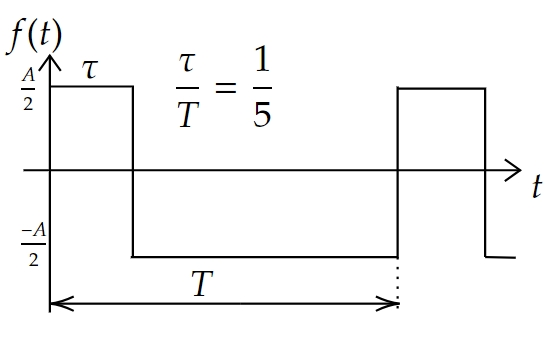
\includegraphics[width=0.4\textwidth]{3.18.1(b).png}
	}
	\subfloat[]{
		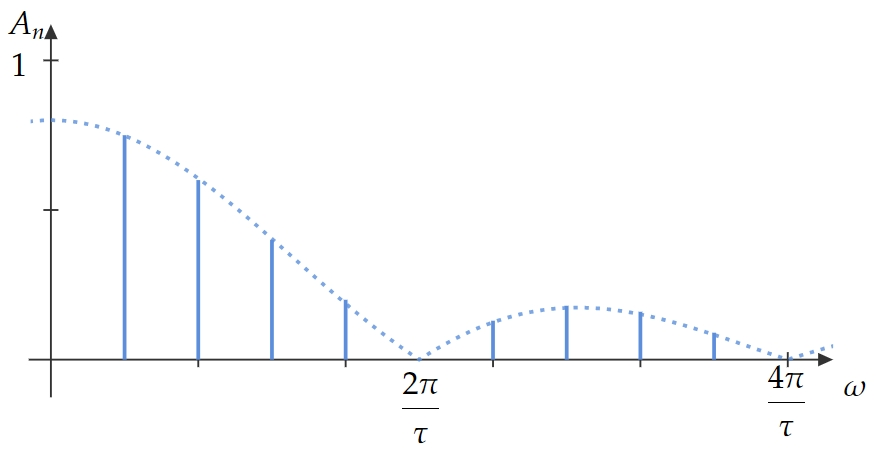
\includegraphics[width=0.45\textwidth]{3.18.1(d).png}
	}
	\caption{}
\end{figure}

\subsection*{二、实验原理}
\begin{enumerate}
  \item 矩形脉冲的频谐与脉冲宽度 $\tau$ 及重复周期 $T$ 之问有着密切的关系,本实验的任务就研究这种关系。测量频谐的方法同实验十四。短形脉冲由数宇信号发生器提供,矩形脉冲的宽度与幅度均用数宇示波器来测量。
  \item 矩形脉冲谐波的幅度是按下式规律变化:
        \begin{equation*}
          A_m = \dfrac{2A\tau}{T}\left |\dfrac{\sin \dfrac{n\pi\tau}{T}}{\dfrac{n\pi\tau}{T}} \right |
        \end{equation*}
        其中 $A_m$ 表示第 $n$ 谐波的幅度,$A$ 表示脉冲的幅度,$\tau$ 表示脉冲宽度,$T$ 表示脉冲重复周期。
        从上式可知,周期性矩形脉冲的频谱有几个重要的特点:
        \begin{enumerate}
          \item[(1)] 频谱包络线的零点仅取決于 $\tau$,而与 $T$ 无关,第一个零点的角频率为 $\dfrac{2\pi}{\tau}$,$\tau$ 越小,则第一个零点的角频率越高。
          \item[(2)] 频谱的密度仅取决于 $T$,而与 $\tau$ 无关,$T$ 越大,则谱线愈密。
          \item[(3)] 谐波的幅度取决于 $A$ 及 $\dfrac{\tau}{T}$,$\dfrac{\tau}{T}$ 愈小,则幅度愈小。
          \item[(4)] 各种周期信号频谱的共同点为:离散性,谐波性和收敛性。
        \end{enumerate}
        由上式可知:谐波的次数及幅度与 $\dfrac{\tau}{T}$ 有关,下面给出了脉冲宽度 $\tau$ 不变,而改变脉冲周期 $T$ 及脉冲周期 $T$ 不变,而改变脉冲宽度 $\tau$,这二种情况下的振幅频谱图如图 $1$ 所示。
\end{enumerate}



\subsection*{三、实验内容及要求}
\begin{enumerate}
  \item 测量重复频率 $f = 20KHz$,脉冲宽度 $\tau$ 与周期 $T$ 之比 $\dfrac{\tau}{T} = \dfrac{1}{5}$,脉冲幅度 $A = 2V$ 的矩形脉冲的频谱,数据记录于表1,并且绘制频谱图于图2。
  \begin{table}[H]
		\renewcommand\arraystretch{1.7}
		\centering
		\caption{$f = 20KHz, \dfrac{\tau}{T} = \dfrac{1}{5}, A = 2V$}
		\begin{tabularx}{\textwidth}{|p{0.2\textwidth}|X|X|X|X|X|X|X|X|X|X|}
			\hline
			谐波频率fn(kHz) & 20 & 40 & 60 & 80 & 100 & 120 & 140 & 160 & 180 & 200 \\
			\hline
			谐波幅度Pn(dB) & -2.7 & -4.8 & -8.3 & -15.1 & -28.2 & -19.6 & -15.5 & -16.7 & -18.4 & -34.8 \\
			\hline
      谐波电压 $U_n = 0.775 \times 10^{\frac{pn}{20}}$ & 0.57 & 0.45 & 0.30 & 0.14 & 0.03 & 0.08 & 0.13 & 0.11 & 0.09 & 0.01 \\
			\hline
		\end{tabularx}
	\end{table}
  \begin{figure}[htbp][H]
    \centering
    \subfloat[]{
      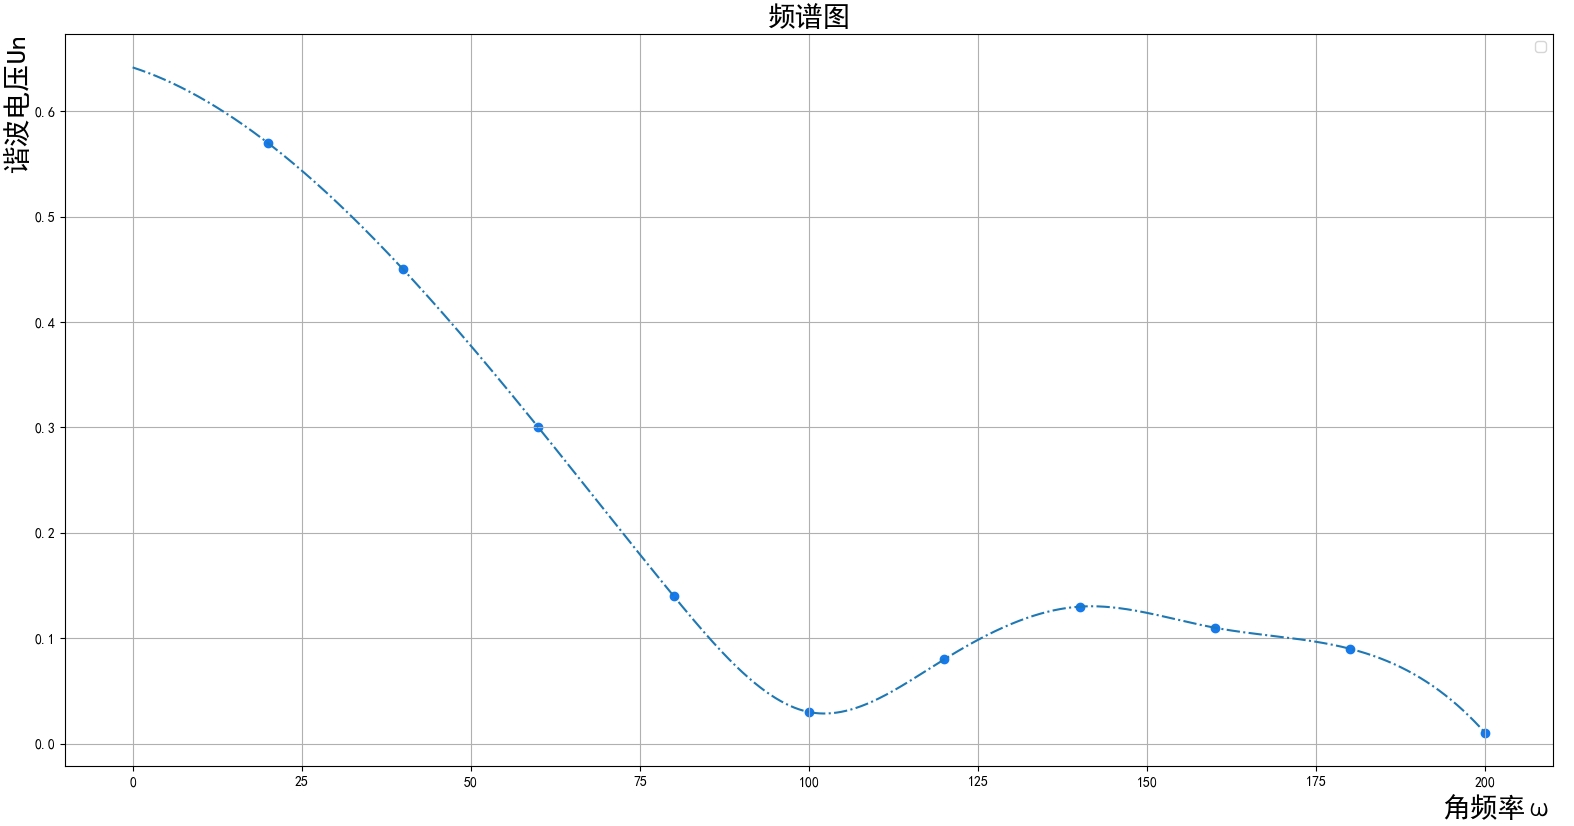
\includegraphics[width=0.5\textwidth]{1-a.png}
    }
    \subfloat[]{
      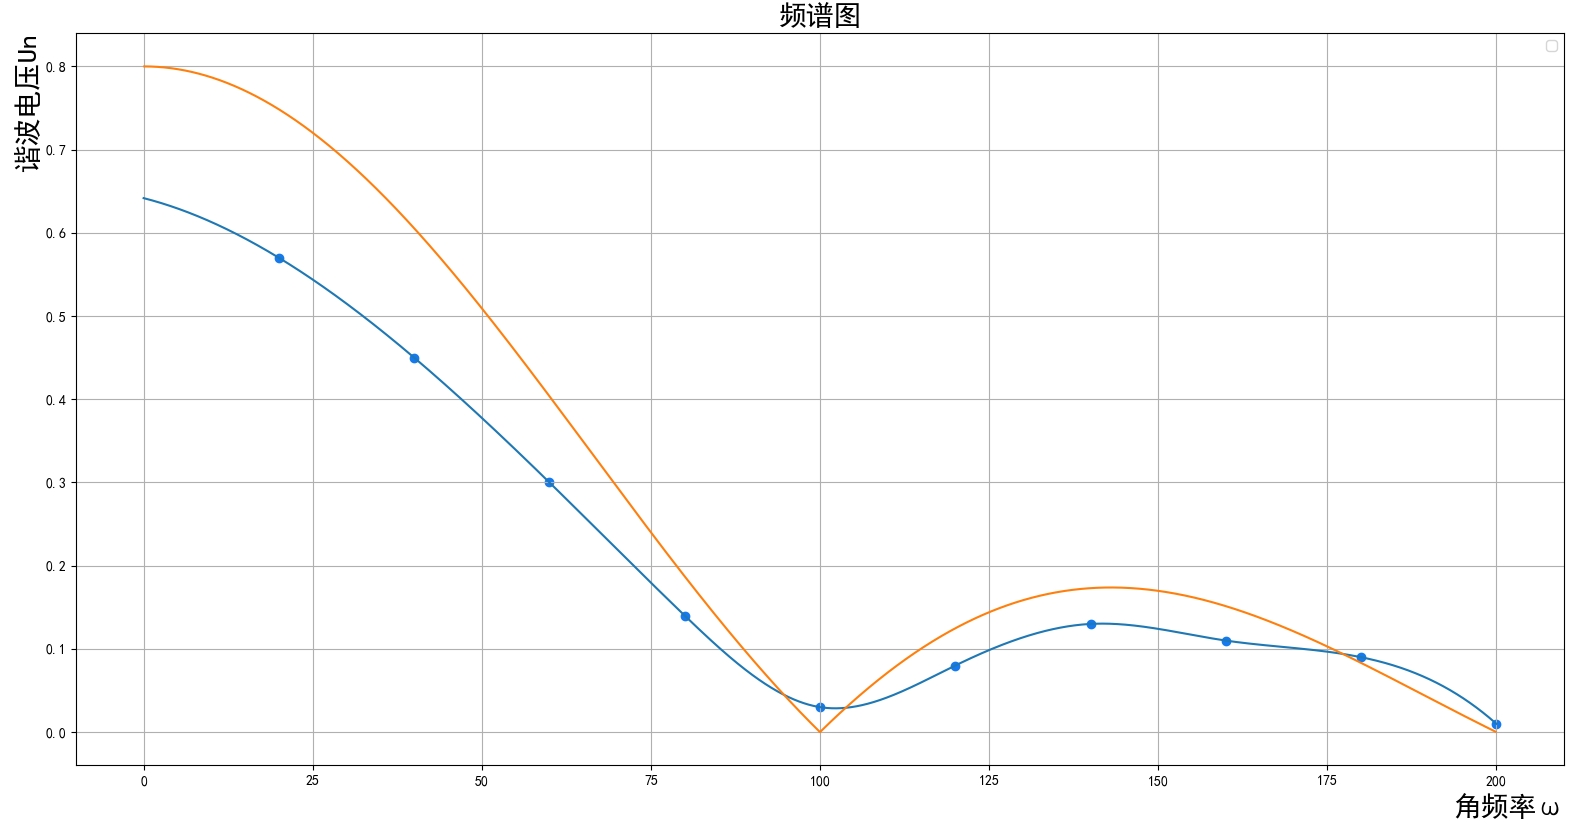
\includegraphics[width=0.5\textwidth]{1-b.png}
    }
    \caption{实际图样以及实际,理想对比图}
  \end{figure}
  \item 测量重复频率 $f = 10KHz$,脉冲宽度 $\tau$ 与周期 $T$ 之比 $\dfrac{\tau}{T} = \dfrac{1}{5}$,脉冲幅度 $A = 2V$ 的矩形脉冲的频谱,数据记录于表2,并且绘制频谱图于图3。
  \begin{table}[H]
		\renewcommand\arraystretch{1.7}
		\centering
		\caption{$f = 10KHz, \dfrac{\tau}{T} = \dfrac{1}{5}, A = 2V$}
		\begin{tabularx}{\textwidth}{|p{0.12\textwidth}|p{1.48em}|p{1.48em}|p{1.48em}|X|X|X|X|X|X|X|X|X|X|X|X|}
			\hline
			谐波频率fn(kHz) & 10 & 20 & 30 & 40 & 50 & 60 & 70 & 80 & 90 & 100 & 110 & 120 & 130 & 140 & 150 \\
			\hline
      
			谐波幅度Pn(dB) & \small{-2.9} & \small{-4.7} & \small{-8.3} & \tiny{-14.9} & \tiny{-51.2} & \tiny{-18.5} & \tiny{-15.7} & \tiny{-16.8} & \tiny{-23.1} & \tiny{-37.7} & \tiny{-24.8} & \tiny{-21.1} & \tiny{-21.4} &\tiny{-30.6} & \tiny{-51.2}\\
			\hline
      谐波电压 $U_n = 0.775 \times 10^{\frac{pn}{20}}$ & 0.56 & 0.45 & 0.30 & 0.14 & 0.002 & 0.09 & 0.13 & 0.11 & 0.054 & 0.01 & 0.045 & 0.07 & 0.06 & 0.02 & 0.002 \\
			\hline
		\end{tabularx}
	\end{table}
  \begin{figure}[htbp]
    \centering
    \subfloat[]{
      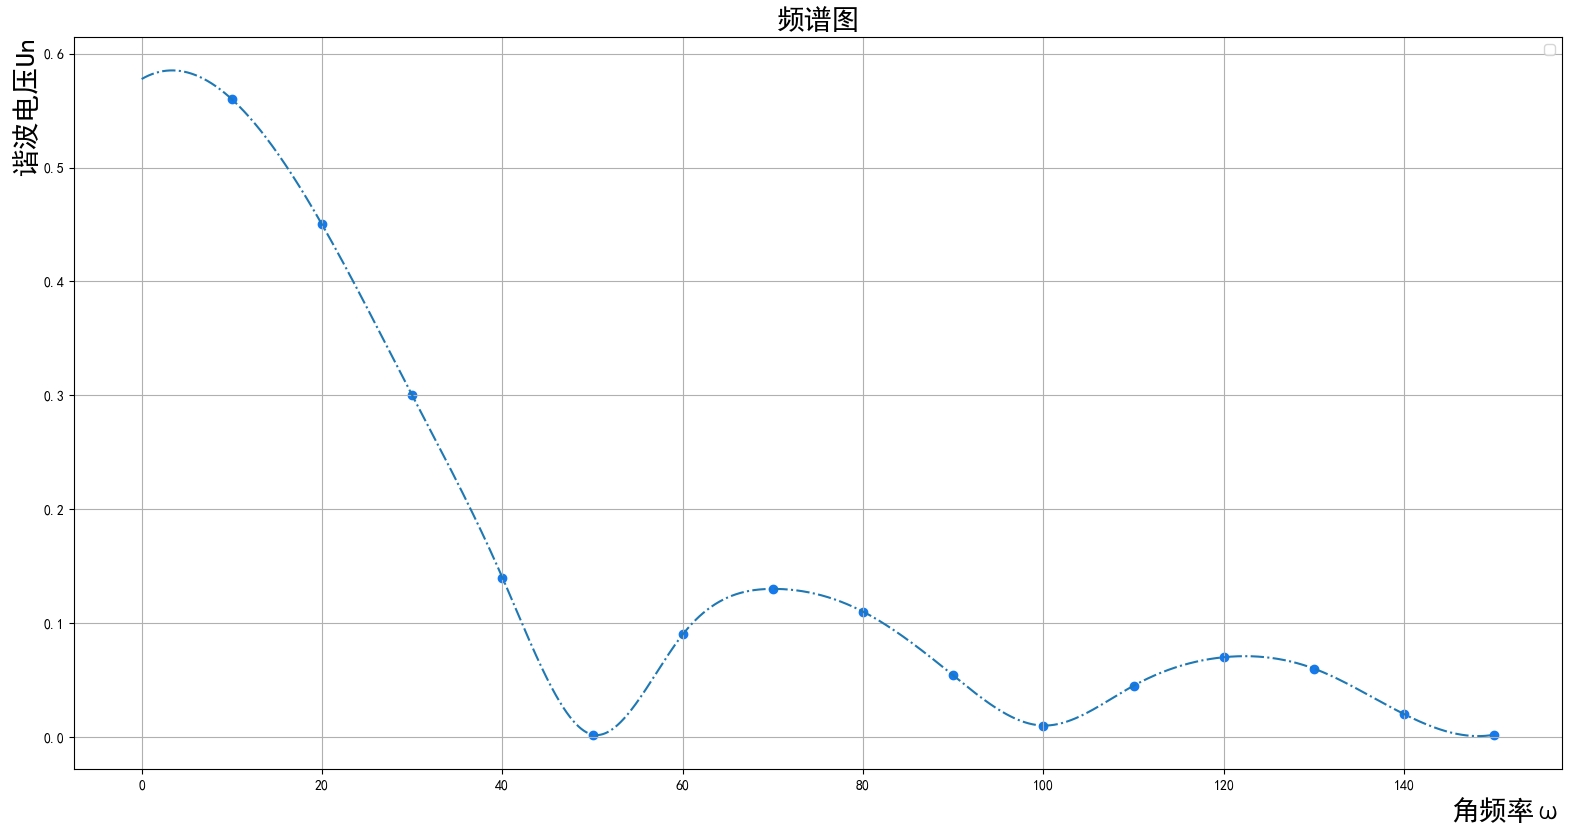
\includegraphics[width=0.5\textwidth]{2-a.png}
    }
    \subfloat[]{
      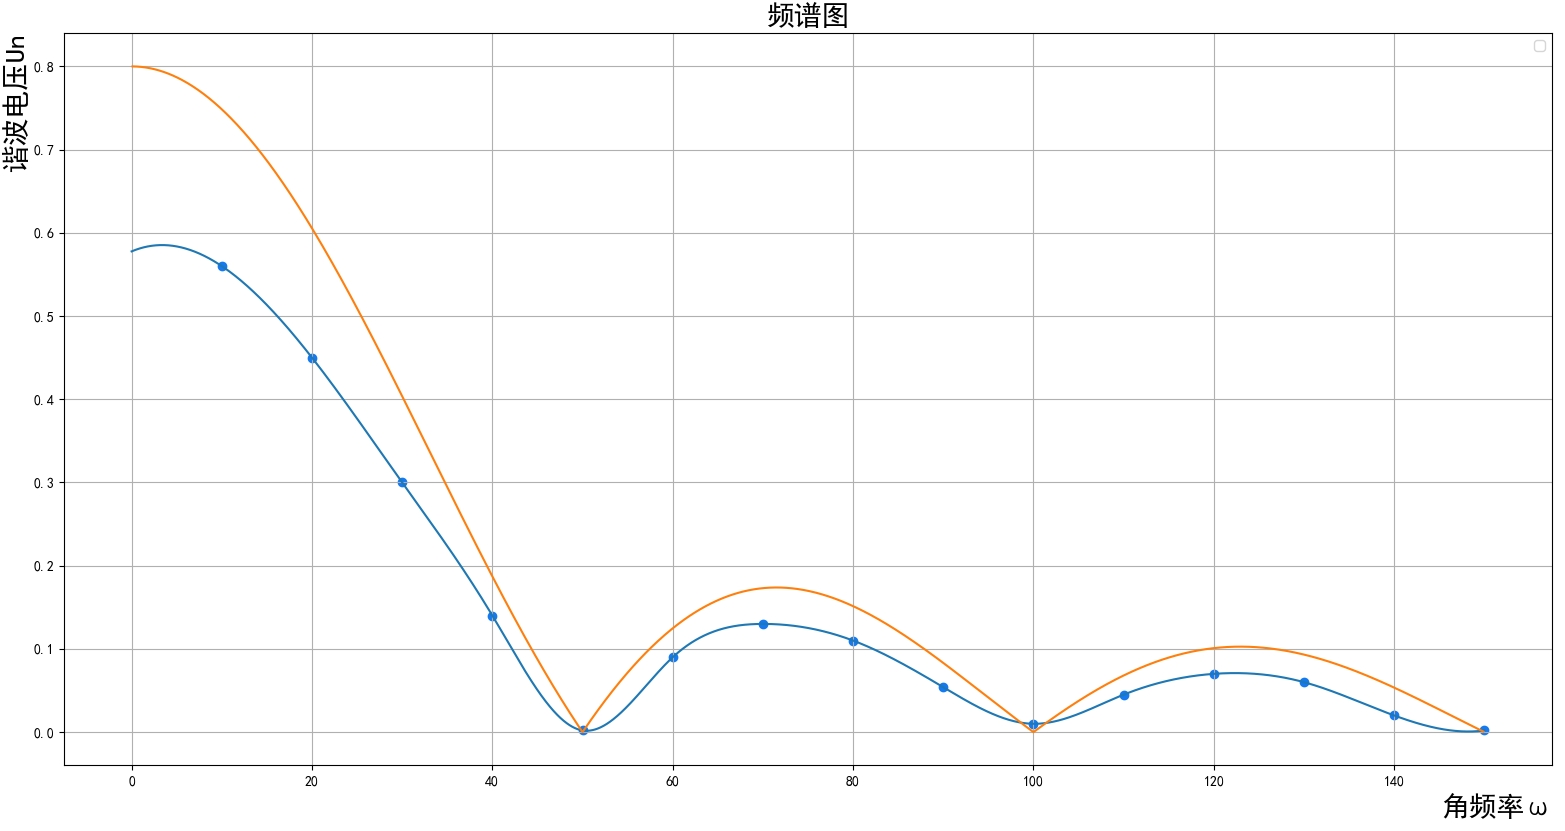
\includegraphics[width=0.5\textwidth]{2-b.png}
    }
    \caption{实际图样以及实际,理想对比图}
  \end{figure}
  \item 测量重复频率 $f = 10KHz$,脉冲宽度 $\tau$ 与周期 $T$ 之比 $\dfrac{\tau}{T} = \dfrac{1}{10}$,脉冲幅度 $A = 2V$ 的矩形脉冲的频谱,数据记录于表3,并且绘制频谱图于图4。
  \begin{table}
		\renewcommand\arraystretch{1.7}
		\centering
		\caption{$f = 10KHz, \dfrac{\tau}{T} = \dfrac{1}{10}, A = 2V$}
		\begin{tabularx}{\textwidth}{|p{0.2\textwidth}|X|X|X|X|X|X|X|X|X|X|}
			\hline
			谐波频率fn(kHz) & 10 & 20 & 30 & 40 & 50 & 60 & 70 & 80 & 90 & 100 \\
			\hline
			谐波幅度Pn(dB) & -8.5 & -8.8 & -9.7 & -10.9 & -12.4 & -14.3 & -17.0 & -20.9 & -26.4 & -38.8 \\
			\hline
      谐波电压 $U_n = 0.775 \times 10^{\frac{pn}{20}}$ & 0.30 & 0.28 & 0.25 & 0.22 & 0.19 & 0.15 & 0.11 & 0.07 & 0.04 & 0.01 \\
			\hline
      谐波频率fn(kHz) & 110 & 120 & 130 & 140 & 150 & 160 & 170 & 180 & 190 & 200 \\
			\hline
			谐波幅度Pn(dB) & -34.6 & -30.7 & -23.8 & -22.8 & -22.9 & -23.6 & -25.3 & -28.2 & -38.5 & -41.7 \\
			\hline
      谐波电压 $U_n = 0.775 \times 10^{\frac{pn}{20}}$ & 0.014 & 0.02 & 0.05 & 0.06 & 0.06 & 0.05 & 0.04 & 0.03 & 0.009 & 0.006 \\
			\hline
		\end{tabularx}
	\end{table}
  \begin{figure}[htbp]
    \centering
    \subfloat[]{
      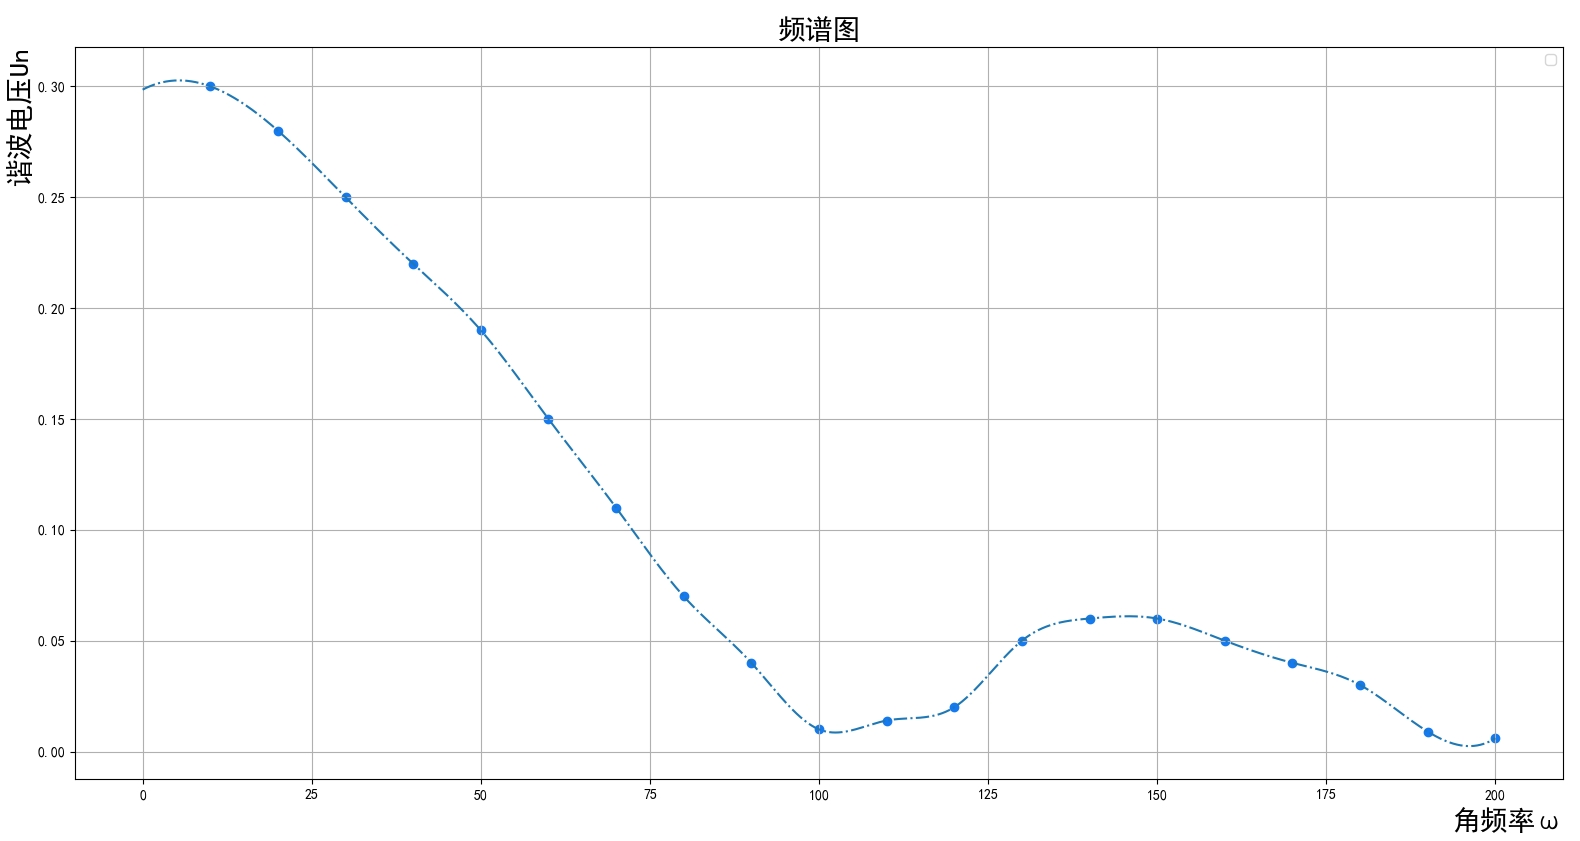
\includegraphics[width=0.5\textwidth]{3-a.png}
    }
    \subfloat[]{
      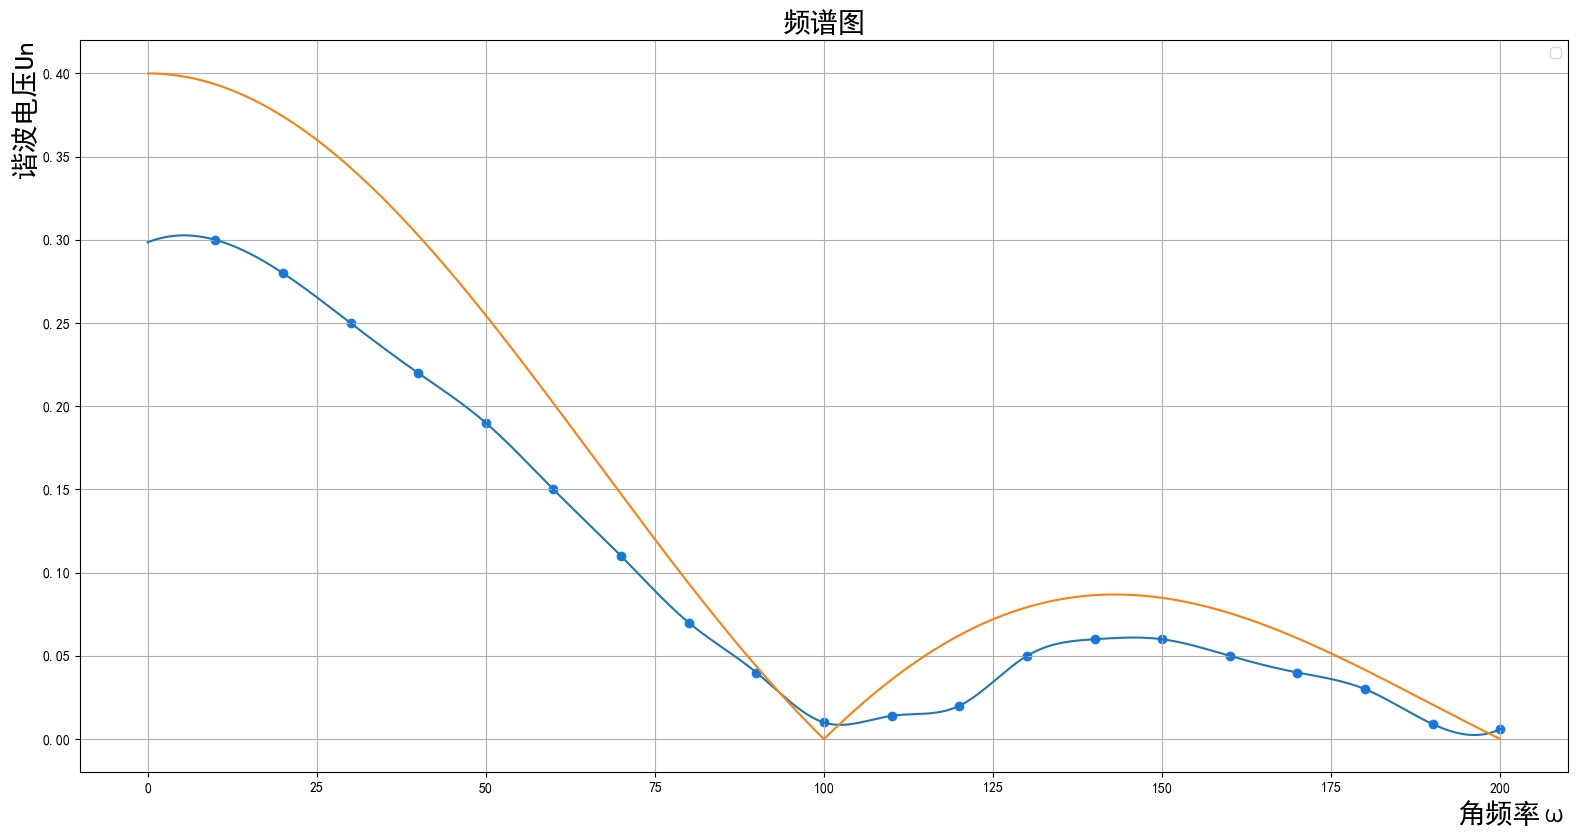
\includegraphics[width=0.5\textwidth]{3-b.png}
    }
    \caption{实际图样以及实际,理想对比图}
  \end{figure}
\end{enumerate}
注:$U_n = 0.775 \time 10^{\frac{P_n}{20}}$

\subsection*{四、数据处理}
  \begin{enumerate}
    \item 理想情况电压的计算过程
      \begin{enumerate}
        \item 重复频率 $f = 20KHz$(即 $f = 20n$ ),脉冲宽度 $\tau$ 与周期 $T$ 之比 $\dfrac{\tau}{T} = \dfrac{1}{5}$,脉冲幅度 $A = 2V$ 的矩形脉冲的频谱,利用公式
          \begin{equation*}
            A_m = \dfrac{2A\tau}{T}\left |\dfrac{\sin \dfrac{n\pi\tau}{T}}{\dfrac{n\pi\tau}{T}} \right |
          \end{equation*}
          代入数值可计算出理想状况:
          \begin{table}[htbp]
            \renewcommand\arraystretch{1.7}
            \centering
            \caption{$f = 10KHz, \dfrac{\tau}{T} = \dfrac{1}{10}, A = 2V$}
            \begin{tabularx}{\textwidth}{|p{0.2\textwidth}|X|X|X|X|X|X|X|X|X|X|}
              \hline
              谐波频率fn(kHz) & 20 & 40 & 60 & 80 & 100 & 120 & 140 & 160 & 180 & 200 \\
              \hline
              理想谐波电压 & 0.75 & 0.61 & 0.40 & 0.19 & $3.1 \times 10^{-17}$ & 0.12 & 0.17 & 0.15 & 0.08 & $3.1 \times 10^{-17}$ \\
              \hline
            \end{tabularx}
          \end{table}
        % \clearpage
        \item 重复频率 $f = 10KHz$(即 $f = 10n$ ),脉冲宽度 $\tau$ 与周期 $T$ 之比 $\dfrac{\tau}{T} = \dfrac{1}{5}$,脉冲幅度 $A = 2V$ 的矩形脉冲的频谱,利用公式
          \begin{equation*}
            A_m = \dfrac{2A\tau}{T}\left |\dfrac{\sin \dfrac{n\pi\tau}{T}}{\dfrac{n\pi\tau}{T}} \right |
          \end{equation*}
          代入数值可计算出理想状况:
          \begin{table}[htbp]
            \renewcommand\arraystretch{1.7}
            \centering
            \caption{$f = 10KHz, \dfrac{\tau}{T} = \dfrac{1}{10}, A = 2V$}
            \begin{tabularx}{\textwidth}{|p{0.2\textwidth}|X|X|X|X|X|X|X|X|X|X|X|X|X|X|X|}
              \hline
              谐波频率fn(kHz) & 10 & 20 & 30 & 40 & 50 & 60 & 70 & 80 & 90 & 100 & 110 & 120 & 130 & 140 & 150 \\
              \hline
              理想谐波电压 & 0.75 & 0.61 & 0.40 & 0.19 & $3.1 \times 10^{-17}$ & 0.12 & 0.17 & 0.15 & 0.08 & $3.1 \times 10^{-17}$ & 0.07 & 0.1 & 0.09 & 0.05 & $3.1 \times 10^{-17}$\\
              \hline
            \end{tabularx}
          \end{table}
        \item 重复频率 $f = 10KHz$(即 $f = 10n$ ),脉冲宽度 $\tau$ 与周期 $T$ 之比 $\dfrac{\tau}{T} = \dfrac{1}{10}$,脉冲幅度 $A = 2V$ 的矩形脉冲的频谱,利用公式
          \begin{equation*}
            A_m = \dfrac{2A\tau}{T}\left |\dfrac{\sin \dfrac{n\pi\tau}{T}}{\dfrac{n\pi\tau}{T}} \right |
          \end{equation*}
          代入数值可计算出理想状况:
          \begin{table}[htbp]
            \renewcommand\arraystretch{1.7}
            \centering
            \caption{$f = 10KHz, \dfrac{\tau}{T} = \dfrac{1}{10}, A = 2V$}
            \begin{tabularx}{\textwidth}{|p{0.2\textwidth}|X|X|X|X|X|X|X|X|X|X|}
              \hline
              谐波频率fn(kHz) & 10 & 20 & 30 & 40 & 50 & 60 & 70 & 80 & 90 & 100 \\
              \hline
              理想谐波电压 & 0.40 & 0.37 & 0.34 & 0.30 & 0.25 & 0.20 & 0.15 & 0.10 & 0.04	& $1.6 \times 10^{-17}$	\\
              \hline
              谐波频率fn(kHz) & 110 & 120 & 130 & 140 & 150 & 160 & 170 & 180 & 190 & 200 \\
              \hline
              理想谐波电压 & 0.036 & 0.062 & 0.079 & 0.086 & 0.085 & 0.076 & 0.061 & 0.042 & 0.021 & $1.6 \times 10^{-17}$\\
              \hline
            \end{tabularx}
          \end{table}
      \end{enumerate}
    \item 第一个零点处角频率的比较
      \begin{enumerate}
        \item 实验一,根据公式 $\omega_0 = \dfrac{2\pi}{\tau}$,代入数据 $\dfrac{\tau}{T} = \dfrac{1}{5}$,$f = 20KHz$,得到 $\omega_0 = \dfrac{2\pi}{\tau} = 2 \times 10^5 \pi$,
        
          实际测量第一个零点频率 $f \approx 1 \times 10^5 \pi$,由 $\omega = 2\pi f$ 可知,与实际测量值比较近似相等。
        \item 实验二,根据公式 $\omega_0 = \dfrac{2\pi}{\tau}$,代入数据 $\dfrac{\tau}{T} = \dfrac{1}{5}$,$f = 10KHz$,得到 $\omega_0 = \dfrac{2\pi}{\tau} = 1 \times 10^5 \pi$,
        
          实际测量第一个零点频率 $f \approx 0.5 \times 10^5 \pi$,由 $\omega = 2\pi f$ 可知,与实际测量值比较近似相等。
        \item 实验三,根据公式 $\omega_0 = \dfrac{2\pi}{\tau}$,代入数据 $\dfrac{\tau}{T} = \dfrac{1}{10}$,$f = 10KHz$,得到 $\omega_0 = \dfrac{2\pi}{\tau} = 2 \times 10^5 \pi$,
        
          实际测量第一个零点频率 $f \approx 1 \times 10^5 \pi$,由 $\omega = 2\pi f$ 可知,与实际测量值比较近似相等。
      \end{enumerate}
  \end{enumerate}

\subsection*{五、实验结论与思考}
  \begin{enumerate}
    \item 矩形脉中频谱包络线的要点仅取决于 $\tau$ ,与 $T$ 无关,且第一个零点角频率为 $\dfrac{2\pi}{\tau}$。$\tau$ 越小,第一个零点角频率越高。
    \item 实际测量值与理论值存在误差,可能是选频电平表未自较,或使用不当或仪器本身误差。
    \item 频谱的密度只与 $T$ 有关,$T$ 越大,谱线越卡密。
  \end{enumerate}
\end{document}


